\documentclass[tikz,border=4pt]{standalone}
\usepackage{amsmath}
\begin{document}
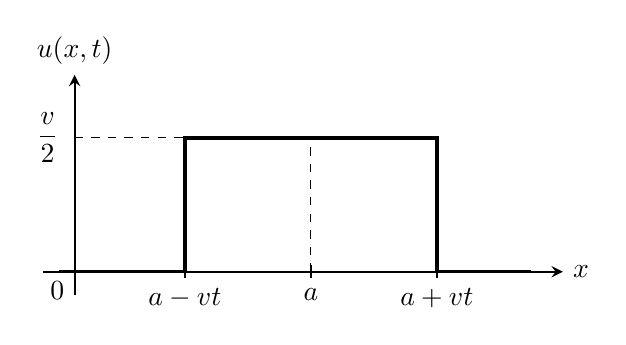
\begin{tikzpicture}[>=stealth, thick, scale=1.0]
  % Axes
  \draw[->] (-0.4, 0) -- (6.2, 0) node[right] {$x$};
  \draw[->] (0, -0.3) -- (0, 2.5) node[above] {$u(x, t)$};
  \node[below left] at (0, 0) {$0$};

  % Rectangular pulse on [a-vt, a+vt] = [1.4, 4.6], center a = 3.0, height v/2 -> y = 1.7
  \draw[very thick] (-0.2, 0) -- (1.4, 0) -- (1.4, 1.7) -- (4.6, 1.7) -- (4.6, 0) -- (5.8, 0);

  % Center a and height v/2
  \draw[dashed, thin] (3.0, 0) -- (3.0, 1.7);
  \draw[dashed, thin] (0, 1.7) -- (1.4, 1.7);
  \node[left] at (-0.08, 1.7) {$\dfrac{v}{2}$};

  % Ticks
  \draw (1.4, 0.08) -- (1.4, -0.08) node[below] {$a - vt$};
  \draw (3.0, 0.08) -- (3.0, -0.08) node[below] {$a$};
  \draw (4.6, 0.08) -- (4.6, -0.08) node[below] {$a + vt$};
\end{tikzpicture}
\end{document}
